%http://matematicazup.com.br/conteudo-matematica-6-ano-ensino-fundamental/
%http://www.cefetsp.br/edu/sertaozinho/professores/Luiz_Carlos_Leal_Junior/622_APOSTILA01_MB.pdf
%http://www.matematica.pt/util/formulas.php Fórmulas
\chapter{Tabuada}
%http://www.estudamos.com.br/jogo_da_memoria/
%http://www.br-ie.org/pub/index.php/sbie/article/view/2516/2174

Mais importante que decorar a tabuada é compreender os padrões utilizados para construí-la. Observe a tabela a baixo. Ela é a conhecida ``grade de multiplicação''. Nela está todas as multiplicações possíveis entre dois números que são maiores ou iguais a um e menores ou iguais a 10. Devido a nosso sistema decimal essa tabuada é o suficiente para que possamos efetuar qualquer outra multiplicação com mais dígitos. Você consegue imaginar o porque isso? Consegue imaginar como utilizá-la para fazer multiplicações com mais de dois dígitos?

\begin{table}[h]
    \centering
    \begin{tabular}{c|c|c|c|c|c|c|c|c|c}
        1  &  2 &  3 &  4 &  5 &  6 &  7 &  8 &  9 & 10\\
        2  &  4 &  6 &  8 & 10 & 12 & 14 & 16 & 18 & 20\\
        3  &  6 &  9 & 12 & 15 & 18 & 21 & 24 & 27 & 30\\
        4  &  8 & 12 & 16 & 20 & 24 & 28 & 32 & 36 & 40\\
        5  & 10 & 15 & 20 & 25 & 30 & 35 & 40 & 45 & 50\\
        6  & 12 & 18 & 24 & 30 & 36 & 42 & 48 & 54 & 60\\
        7  & 14 & 21 & 28 & 35 & 42 & 49 & 56 & 63 & 70\\
        8  & 16 & 24 & 32 & 40 & 48 & 56 & 64 & 72 & 80\\
        9  & 18 & 27 & 26 & 45 & 54 & 63 & 72 & 81 & 90\\
        10 & 20 & 30 & 40 & 50 & 60 & 70 & 80 & 90 & 100\\
    \end{tabular}
    \caption{Grade de múltiplicação}
    \label{tab:my_label}
\end{table}

\begin{itemize}
\item Você notou algum padrão interessante na tabela acima?
\item Como ela poderia ser útil para outras situações?
\item Você consegue encontrar nela a tabuada do 7? e a do 9?
\item Quais estratégias você tomaria para refazer essa tabela caso fosse necessário?
\item Reconstrua a tabela a partir dos padrões que você identificou.
\item Existe outros padrões que podem ser utilizados para reconstruir a grade?
\end{itemize}

%%%%%%%%%%%%%%%%%%%%%%%%%%%%%%%%%%%%%%%%
%\newpage
%\begin{multicols}{2}





\section{Como obter as tabuadas isoladamente}

\subsection{Tabuada do 1, do 5 e de 10}

A tabuada do $1$ e de $10$ seguem o mesmo padrão com a diferença de apenas um zero. Analisando primeiro a tabuada do $1$ notamos que de alguma forma ele não altera o número pelo qual estou multiplicando. Note que o zero faz o mesmo na adição, ambos não alteram o valor com qual estão interagindo. Essa característica vem de uma propriedade das operações chamada ``termo neutro''. 

Olhando para a tabuada do $10$ teremos apenas a característica básica da construção da base decimal. Múltiplicar por dez equivale apenas a aumentar um zero. O detalhe por trás dessa múltiplicação está no trabalho com a vírgula que separa a parte inteira da parte decimal. Será melhor verificado isso quando se estudar as potências de $10$ e a notação científica.

Para o caso da tabuada do $5$ basta somar de cinco em cinco para totalizar o valor procurado. Note que um número multiplicado por $5$ só pode terminar ou em zero, quando o número por par, ou em cinco, quando o número for impar. Acredito que a tabuada do $5$ seja a terceira mais fácil depois das duas tabuadas citadas acima.

\subsection{Tabuada do 2, do 4 e do 8}

Note na grade de múltiplicação que as tabuadas dos números pares são todos pares enquanto a tabuada dos números impares alterna entre impares e pares. Isso ocorre porque multiplicar um número par por outro inteiro resulta em outro número par.

No cado da tabuada do $2$ basta somar cada valor da tábua do $1$ a si mesmo e obteremos a tabuada do dois. Ou seja, multiplicar por dois é o mesmo que somar um número a si mesmo. 

\begin{align*}
    2\times n=n+n
\end{align*}

Note ainda que cada termo da tabuada do $1$ é metade do da tabuada do $2$.

Para obter a tabuada do $4$ basta fazer o mesmo com a tabuada do $2$. Caso se queira a múltiplicação de $4$ por algum número basta dobrar esse número e depois somá-lo consigo mesmo. Ou seja:

\begin{align*}
    4\times n=2\times n+2\times n
\end{align*}

Por exemplo, quanto é $4\times 7$? Ora, primeiro vamos dobrar o $7$, que é $14$, depois basta somar $14+14$ e obteremos $28$. Isso funciona porque dois é metade de quatro. Além disso temos que multiplicar um número por quatro é o mesmo que somar quatro parcelas iguais daquele número.

\begin{align*}
    4\times n&=n+n+n+n\\
    &=(n+n)+(n+n)\\
    &=2\times n+2\times n
\end{align*}

O que justifica isso é a propriedade da associação da soma. Poderiamos também utilizar a propriedade da distribuição como vemos abaixo

\begin{align*}
    4\times n&=(2+2)\times n\\
    &=2\times n+2\times n.
\end{align*}

Note que tudo o que fizemos do $4$ em relação ao $2$ vale, pelos mesmos motivos e da mesma forma do $8$ em relação ao $4$. Para multiplicar algum número por $8$ podemos somar duas parcelas dele multiplicado por quatro. Digamos que temos que calcular quanto é $8\times 9$, ora, basta fazer

\begin{align*}
    8\times9=4\times 9+4\times9.
\end{align*}

Caso não sabendo de cabeça quanto é quatro vezes nove, então apliamos novamente essa propriedade

\begin{align*}
    4\times9&=2\times 9+2\times9\\
    &=18+18=36.
\end{align*}

Voltando para o caso original, teremos

\begin{align*}
    8\times9=36+36=72
\end{align*}

\subsection{Tabuada do 3 e do 6}

Note que multiplicar um número por $3$ é o mesmo que somar esse número consigo mesmo três vezes, ou seja

\begin{align*}
    3\times n=n+n+n.
\end{align*}

Ora, podemos calcular de cabeça esse valor ou podemos achar o dobro dele e somar mais uma parcela. Note que podemos agrupar duas parelas na expressão acima para obtermos

\begin{align*}
    3\times n&=(n+n)+n\\
    &=2\times n+n
\end{align*}

Note que para efetuar a multiplicação de um número por $6$ basta executar o mesmo processo que efetuamos quando estavamos calculando a multiplicação por $4$ regredindo a $2$ e por $8$ regredindo a $4$. Você consegue imaginar como fazer isso, por exemplo, na multiplicação $6\times 7$?

\subsection{Tabuada do 9}

A tabuada do 9 pode ser obtida de algumas fórmas diferentes. A primeira é aquela que ao conhecer você pensa: ``Por que nunca me ensinaram isso na escola''. 

Passo 1: Escreva os números de 0 a 9. Depois de novamente só que em ordem inversa conforme a tabela abaixo.

\begin{center}
\begin{tabular}{c|c|c|c|c|c|c|c|c|c}
09 & 18 & 27 & 36 & 45 & 54 & 63 & 72 & 81 & 90 \\
\end{tabular}
\end{center}


Pronto. Temos nossa tabuada do 9 completa. Essa construção só é verificada na tabuada do 9. Não dá para fazer isso com as outras tabuadas.

Isso ocorre pois ao ``pularmos'' da multiplicação $9\times3$ para a $9\times4$ estamos acrescentando uma parcela de 9. Note que somar 9 é o mesmo que somar 10 e subtrair 1. Isso significa que aumentamos 1 unidade na casa das dezenas e retiramos uma unidade da cada das unidades. Utilizamos aqui da propriedade associativa da múltiplicação.

Com essa ideia partimos para o segundo método.

\subsection{Tabuada dos 9 de termos isolados}

Aqui encontramos de forma isolada os produtos da tabuada do 9. 

A ideia é subtrair 1 do número com quem 9 está sendo multiplicado e acrescentar o que falta para totalizar 9 nas unidades.

Exemplo.

$$9\times5=$$

Agora subtraimos uma unidade do 5 e pomos como dezena.

$$9\times5=4$$

Note que a diferença de 4 para 9 é de 5. Esse valor serão as unidades.

$$9\times5=45.$$

Tente com os demais valores e verifique que é verdadeiro.

Essa propriedade é verificada quando lembramos do famozo nove's fora. $7\times6=42$. Noves fora é $4+2=6$. Quando fazemos isso com a tabuada do 9 temos que todos os nove's fora dão zero. Para verificar basta notar que os nove's fora tiram parcelas de 9 em 9 até o número ser algo entre 0 e 8. No caso das números da tabuada de 9 retirar parcelas de 9 em 9 vai sempre zerar o resultado final.

Note que seria o mesmo que $5\times9$ pela propriedade da comutação da multiplicação.

\subsection{E a tabuada do 7?}

Para os que se perguntarem pela tabuada do $7$, notem que ela já apareceu dentro de todas as outras tabuadas já citadas acima. Graças a propriedade da comutatividade da multiplicação podemos verificar que multiplicar sete por um número é o mesmo que multiplicar esse mesmo número por 7.

\begin{center}
\begin{tabular}{c|c}
 $7\times1=07$    &  $1\times7$\\
  $7\times2=14$   &$ 2\times7$\\
 $ 7\times3=2$1 &$ 3\times7$\\
  $7\times4=28$ & $4\times7$\\
\end{tabular}
\end{center}

Note que o único valor dela que não se encontra nesse método é o $7\times7=49$.


%\end{multicols}

\section{Como utilizar a tabuada para efetuar divisões?}

Observe o exemplo abaixo:
\begin{figure}[h]
   \centering
    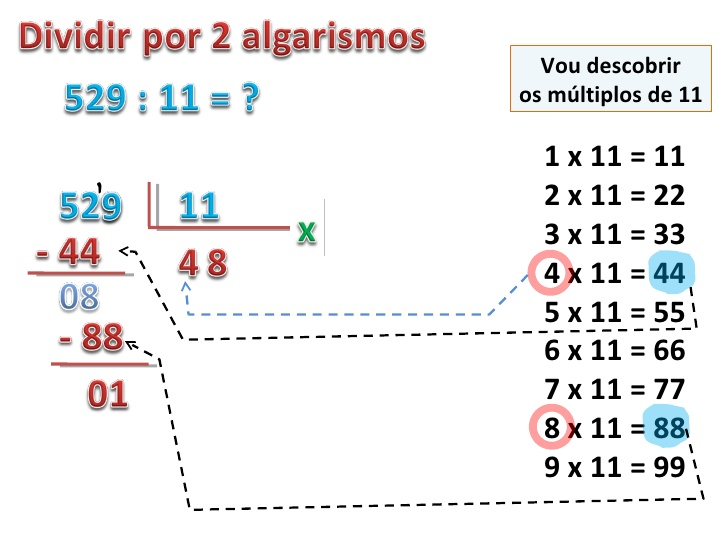
\includegraphics[scale=.4]{./imagens/18.jpg}
    \caption{Tabuada na Divisão}
    \label{fig:my_label}
\end{figure}

Veja que para efetuar a divisão de 529 por 11 precisamos recorrer a tabuada do 11 para completá-la. Isso significa que a tabuada não é só muito importante para que se conheça os múltiplos dos números como também auxíliam para facilitar o processo de divisão, principalmente se for uma divisão com dois ou mais dígitos.


